\documentclass[border=10pt]{standalone}
\usepackage{pgfplots}
\usepgfplotslibrary{colormaps}
\pgfplotsset{compat=1.18}

\begin{document}
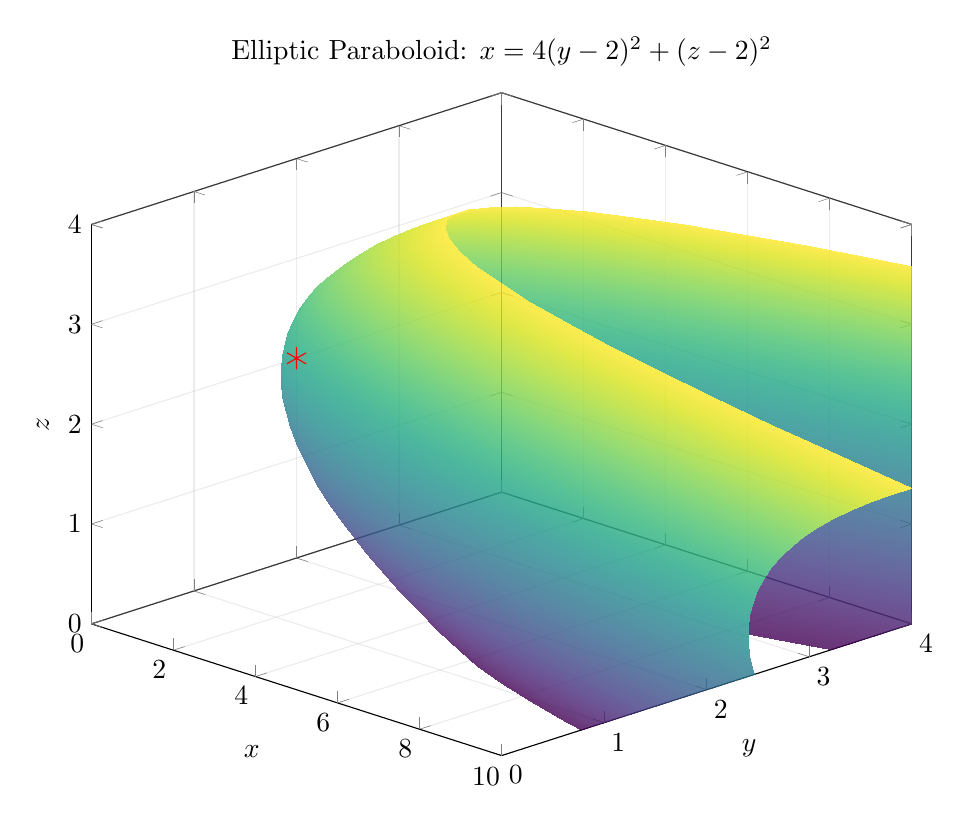
\begin{tikzpicture}
\begin{axis}[
    width=12cm,
    height=10cm,
    xlabel=$x$,
    ylabel=$y$,
    zlabel=$z$,
    title={Elliptic Paraboloid: $x = 4(y-2)^2 + (z-2)^2$},
    view={45}{25},
    colormap/viridis,
    grid=major,
    grid style={opacity=0.3},
    zmin=0, zmax=4,
    ymin=0, ymax=4,
    xmin=0, xmax=10,
]
\addplot3[
    surf,
    domain=0:4,
    y domain=0:4,
    samples=30,
    opacity=0.8,
    shader=interp,
] ({4*(y-2)^2 + (x-2)^2}, y, x);
% Mark vertex
\addplot3[only marks, mark=asterisk, mark size=4pt, red] coordinates {(0,2,2)};
\end{axis}
\end{tikzpicture}
\end{document}